\documentclass[xcolor=table]{beamer}
\usepackage{fontspec}
\usepackage{natbib}
\usepackage{gb4e} 
\usepackage[table]{xcolor}
\usepackage{booktabs} 
%\usepackage{color}
\usepackage{graphicx}
\usepackage{bibentry}
\usepackage{tikz}
\usetikzlibrary{trees}

% \setmainfont[Mapping=tex-text]{Charis SIL}
\let\sfdefault\rmdefault
%\newcommand{\racine}[1]{\begin{math}\sqrt{#1}\end{math}} 
\newfontfamily\phon[Mapping=tex-text,Ligatures=Common,Scale=MatchLowercase,FakeSlant=0.3]{Charis SIL} 
\newcommand{\ipa}[1]{{\phon \mbox{#1}}} %API tjs en italique
\newcommand{\grise}[1]{\cellcolor{lightgray}\textbf{#1}} 
\newcommand{\ra}{$\Sigma_1$} 
\newcommand{\rc}{$\Sigma_3$} 
\newcommand{\ro}{$\Sigma$} 
\newfontfamily\cn[Mapping=tex-text,Ligatures=Common,Scale=MatchUppercase]{MingLiU}%pour le chinois
\newcommand{\zh}[1]{{\cn #1}}


 \begin{document}

 \title{Linguistique panchronique: terrain, formalisation et implémentation}
 \author{Guillaume Jacques}
 \date{}
 \maketitle


 \begin{frame} 
 \frametitle{Publications additionnelles}
 \bibliographystyle{unified}
   \nobibliography{bibliogj.bib}
   \small
\begin{itemize}
\item  \bibentry{jacques14ergative}  
\item  \bibentry{jacques15sr}  
\item  \bibentry{jacques15causative}
\item  \bibentry{jacques15spontaneous}
\item  \bibentry{jacques15derivational.khaling}
\end{itemize}
 \end{frame}
 
    \begin{frame} 
 \frametitle{Plan} 
 
 \begin{itemize}
\item  Recherches précédentes
\item  Programme de recherche
\item  Direction de thèses
\end{itemize}
   \end{frame} 
 
 
   \begin{frame} 
 \frametitle{Recherches précédentes} 
 \begin{itemize}%[<+->]
\item   Empirique (langues sino-tibétaines)
\begin{itemize}
\item Langues anciennes
\item Linguistique de terrain 
\end{itemize}
\item   Théorique
\begin{itemize}
\item Linguistique historique
\item Typologie
\end{itemize}
\end{itemize}
   \end{frame} 
   
   \begin{frame} 
 \frametitle{Langues anciennes} 
 \begin{itemize}%[<+->]
\item Chinois ancien, tibétain ancien, tangoute
\item \bibentry{jacques00ywij}  
\item \bibentry{jacques14tangoute}  
\end{itemize}
   \end{frame} 
   
   \begin{frame} 
 \frametitle{Linguistique de terrain} 
 \begin{itemize}%[<+->]
\item Japhug (2002-présent) (Corpus de 60h de textes)
\item Khaling (2011-présent)
\item Stau (2012-présent)
\item Zbu (2003)
\item Chang naga (2007)
\item Tibétain de Tchoné (2010) 
\item Pumi (2008-2009)
\end{itemize}
   \end{frame} 
   
      \begin{frame} 
 \frametitle{Linguistique de terrain} 
  \framesubtitle{Japhug} 
    \begin{figure}[H]
\centering
\includegraphics[height=50mm]{carte.JPG}
\end{figure}   
       \end{frame} 
       
      \begin{frame} 
 \frametitle{Linguistique de terrain} 
  \framesubtitle{Japhug} 
 \begin{itemize}%[<+->]
\item Dictionnaire multimédia (juin 2015)
\item \bibentry{jacques10gesar}
\item \bibentry{jacques08}  
\item une dizaine d'articles sur la morphosyntaxe, parus dans \textit{Lingua}, \textit{Linguistic Typology}, \textit{Anthropological Linguistics}, \textit{LTBA}
\end{itemize}
    \end{frame} 
    
      \begin{frame} 
 \frametitle{Linguistique de terrain} 
  \framesubtitle{Khaling} 
  \begin{itemize}%[<+->]
\item Dictionnaire multimédia des verbes (juin 2015)
\item \bibentry{jacques12khaling}  
\item \bibentry{jacques14auditory}
\end{itemize}
    \end{frame} 
    
   \begin{frame} 
 \frametitle{Linguistique historique} 
 
 Linguistique diachronique néo-grammairienne et linguistique panchronique (Sino-tibétain, indo-européen, sémitique, algonquien, turcique)
  \small
 \begin{itemize}%[<+->]
\item \bibentry{jacques.michaud11naish}  
\item \bibentry{jacques11lingua}  
\item \bibentry{jacques13arapaho}  
\end{itemize}
   \end{frame} 
   
   \begin{frame} 
 \frametitle{Typologie} 
 
 Théorie de la grammaticalisation, typologie des marques de voix, du mouvement associé, des systèmes d'indexation polypersonnels
 \small
 \begin{itemize}%[<+->]
\item \bibentry{jacques12incorp}  
\item \bibentry{jacques13harmonization}  
\item \bibentry{jacques14antipassive}  
\item \bibentry{antonov14need}  
\end{itemize}
   \end{frame} 
    
  \begin{frame} 
 \frametitle{Projet de recherche} 
 
  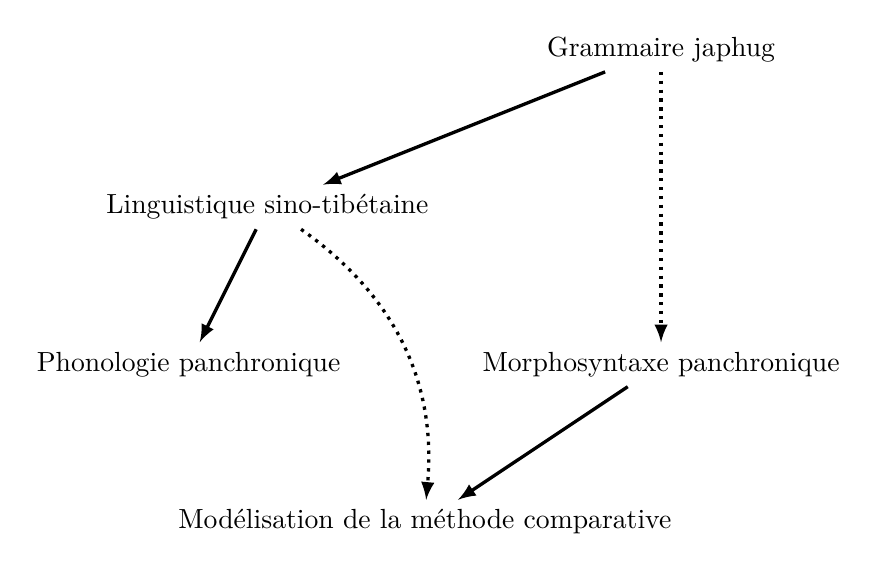
\begin{tikzpicture}
    \node (C) at (2,-1) {Grammaire japhug};
        \node (D) at (-3,-3)  {Linguistique sino-tibétaine};
       \node (F) at (-4,-5)  {Phonologie panchronique};%\\ Adversative};
        \node (G) at (2,-5) {Morphosyntaxe panchronique}; 
             \node (H) at (-1,-7)  {Modélisation de la méthode comparative};
  %  \node (J) at (-0.5,-9) {\textbf{Comparee NP}};
    
    
\tikzstyle{peutetre}=[->,dotted,very thick,>=latex]
\tikzstyle{sur}=[->,very thick,>=latex]
\draw[sur] (C)--(D);
\draw[sur] (D)--(F);
\draw[sur] (G)--(H);
\draw[peutetre] (C)--(G);
\draw[peutetre] (D) to[bend left] (H);
%\draw[peutetre] (C) to[bend right] (F);

\end{tikzpicture}

   
  \end{frame}   

   \begin{frame} 
 \frametitle{Grammaire Japhug} 
 \begin{itemize}%[<+->]
 \item 2015-2016: publication d'une dizaine d'articles
\item 2017-2019: rédaction de la grammaire
\end{itemize}
   \end{frame} 
   
   \begin{frame} 
 \frametitle{Linguistique comparative des langues sino-tibétaines} 
 \begin{itemize}%[<+->]
 \item Phylogénie du sino-tibétain
  \item Dictionnaire comparatif des langues rgyalronguiques et des kiranties
  \item Phonologie et morphologie comparées du sino-tibétain
 \item Diversité typologique de la famille 
\end{itemize}
   \end{frame} 

   \begin{frame} 
 \frametitle{Phonologie panchronique} 
 \begin{itemize}%[<+->]
 \item Unidirectionnalité des changements phonétiques
 \item Changements de lieu d'articulation dans les systèmes consonantiques
\end{itemize}
   \end{frame} 

   \begin{frame} 
 \frametitle{Morphosyntaxe panchronique} 
 \begin{itemize}%[<+->]
 \item Évidentialité nominale (article pour le Oxford Handbook of Evidentiality)
 \item Systèmes d'indexation (algonquien, sino-tibétain)
 \item Évolution des systèmes de voix
 \item Typologie des langues OV préfixantes (athabasque, sioux, sino-tibétain)
\end{itemize}
   \end{frame} 

   \begin{frame} 
 \frametitle{Modélisation de la méthode comparative} 
 \begin{itemize}%[<+->]
 \item  Implémentation en transducteurs à état fini des changements phonétiques
  \item Application de la \textit{minimal description length} en morphologie et en linguistique pour mesurer la complexité relative d'hypothèses concurrentes
  \item Modélisation de l'analogie
\end{itemize}
   \end{frame} 

  \begin{frame} 
 \frametitle{Direction de doctorants} 

\begin{enumerate}
\item Gong Xun (Zbu)
\item Lai Yunfan (Khroskyabs)
\item Gao Yang (Menya)
\item Rao Min (Guiqiong)
\end{enumerate}
 \small
\begin{itemize}
\item  \bibentry{lai13fuyin}
\item  \bibentry{gongxun14agreement}  
\item  \bibentry{lai14person}
\end{itemize}   
  \end{frame}   

\end{document}